`% !TeX root = ../defense.tex

\section{Data Preparation}
\frame{\sectionpage}


\begin{frame}{Corpus}
    \begin{enumerate}[<+->]\itemsep9pt
      \item Switchboard corpus (NXT).
      \item Audio recording of casual conversations between randomly chosen speakers.
      \item 2483 conversation, involving 520 speakers
      \item In our research the corpus contain 642 conversations.
    \end{enumerate}

\end{frame}{}


\begin{frame}{Preprocessing pipeline}
\begin{figure}[ht!]
\centering
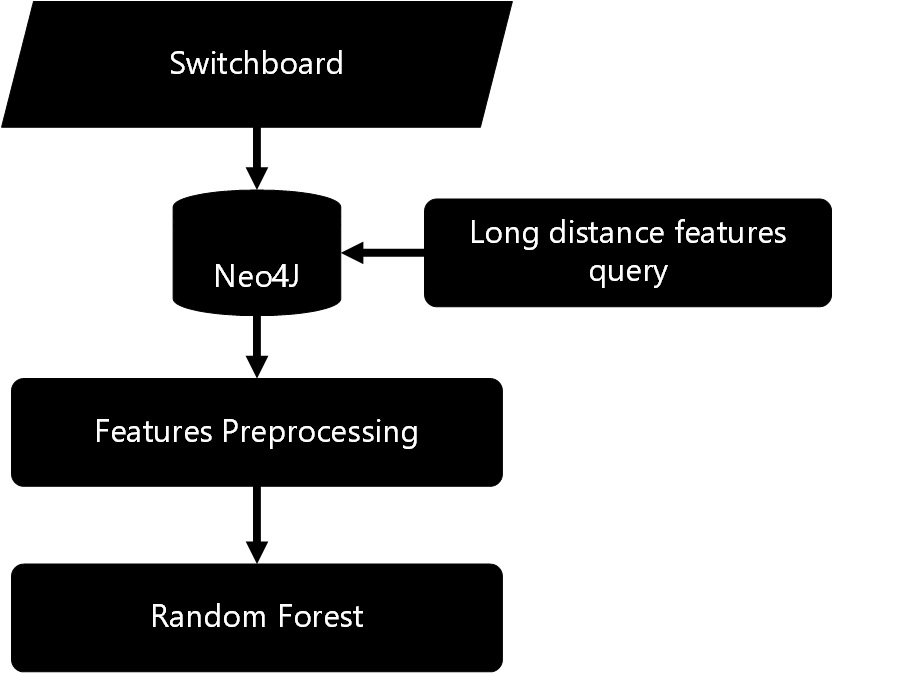
\includegraphics[width=20em]{../latex/pipeline.jpg}\vspace{-1em}
\end{figure}
\end{frame}


\begin{frame}{Conversation representation}
\begin{figure}[ht!]
\centering
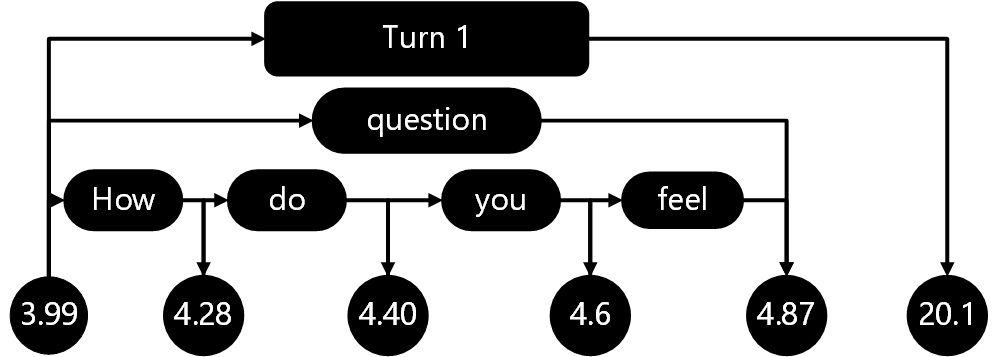
\includegraphics[width=30em]{../latex/graph5.jpg}\vspace{-1em}
\end{figure}
\end{frame}



\begin{frame}{Preprocessing}
 \begin{itemize}
    \item Removed 11 dialogue acts that were coded as other in switchboard.
    \item Skip the first 120 seconds of the conversation.
      \begin{itemize}
      \item Gives time for conversant to form the conversional image.
      \item Reduces the dialogue acts from 50633 to 37508.
      \end{itemize}
    \item Reduce data sparsity by collapsing 65 dialog acts into 9.
  \end{itemize}

  \begin{table}
     \begin{center}
     \begin{tabular}{l | l}
    \hline
Switchboard dialog acts &  Dialog act classes  \\
    \hline
sd,h,bf      & statement   \\
sv,ad,sv@    & statement - opinion  \\
aa,aa\^r     & agree accept \\
\%.\%-,\%@   & abandon      \\
b,bh         & backchannel  \\
qy,qo,qh     & question     \\
no,ny,ng,arp & answer       \\
+            & +            \\
o@,+@        & NA           \\
  \hline
\end{tabular}
\end{center}\vspace{-0.5em}
\caption{Mapping from dialog act to dialog act class}
\label{tab:mapping}
\end{table}

\end{frame}{}


\section{Data Exploration}
\frame{\sectionpage}



\begin{frame}{Dialog act relative count}
\begin{figure}[ht!]
\centering
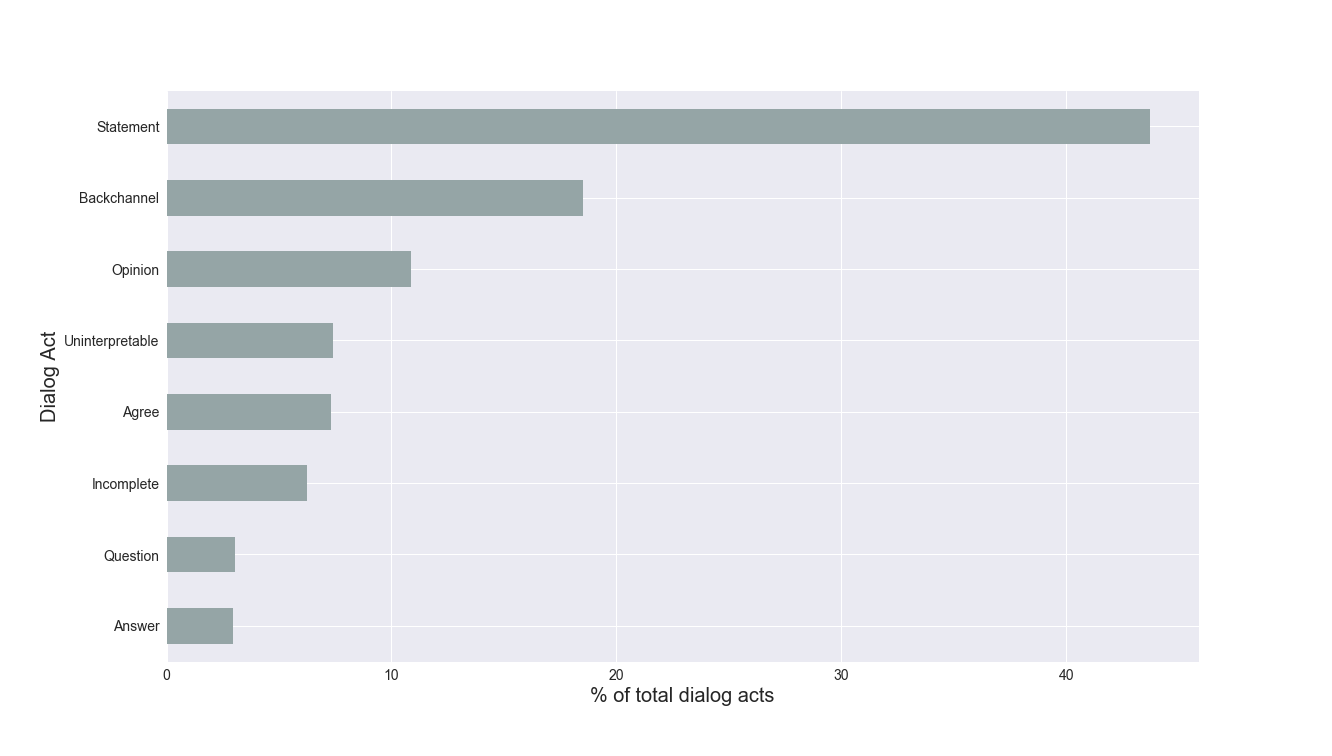
\includegraphics[width=36em]{../scikitlearn/figures/f1.png}\vspace{-1em}
\end{figure}
\end{frame}

\begin{frame}{Turn Length Distribution}
\begin{figure}[ht!]
\centering
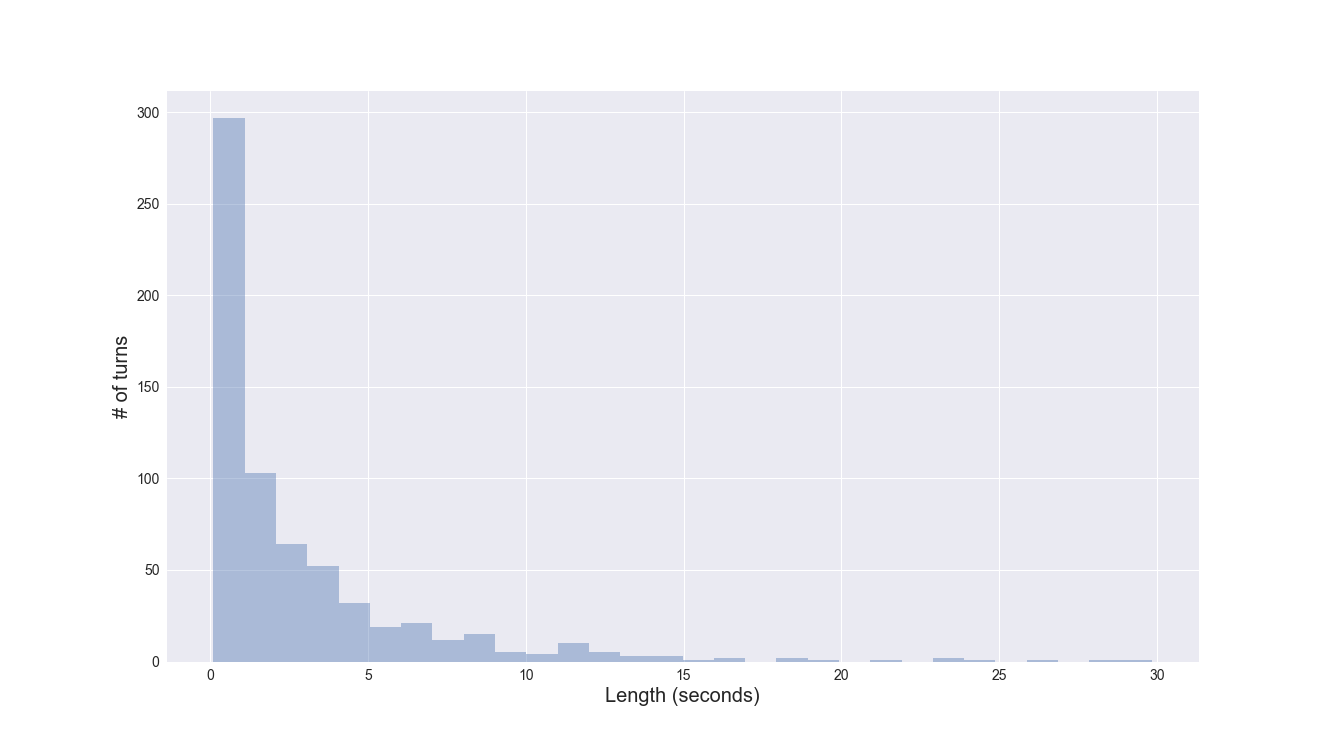
\includegraphics[width=36em]{../scikitlearn/figures/f10.png}\vspace{-1em}
\end{figure}
\end{frame}



\begin{frame}{Dialog act probability of turn change}
\begin{figure}[ht!]
\centering
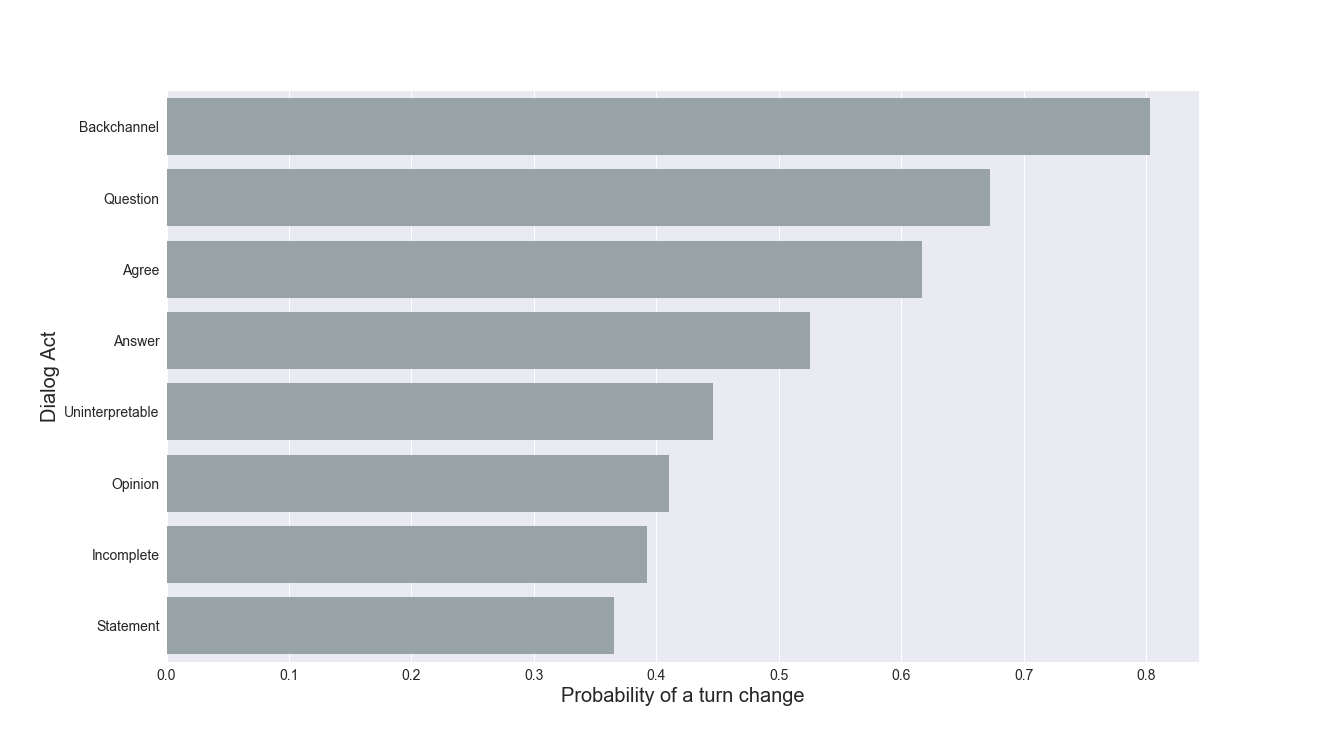
\includegraphics[width=36em]{../scikitlearn/figures/f2.png}\vspace{-1em}
\end{figure}
\end{frame}



\begin{frame}{Relative Turn Length effect on probability of turn change}
\begin{figure}[ht!]
\centering
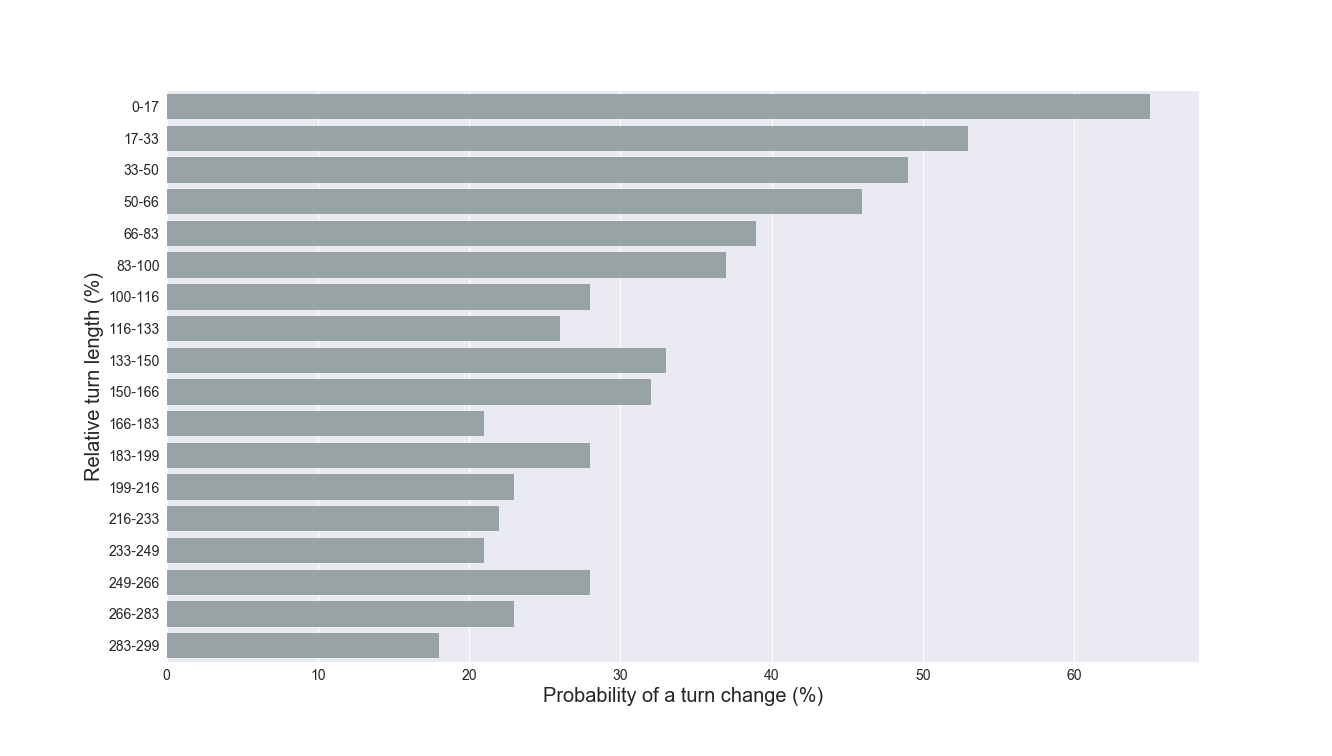
\includegraphics[width=36em]{../scikitlearn/figures/f5.png}\vspace{-1em}
\end{figure}
\end{frame}

\begin{frame}{Relative Turn Control effect on probability of a turn change}
\begin{figure}[ht!]
\centering
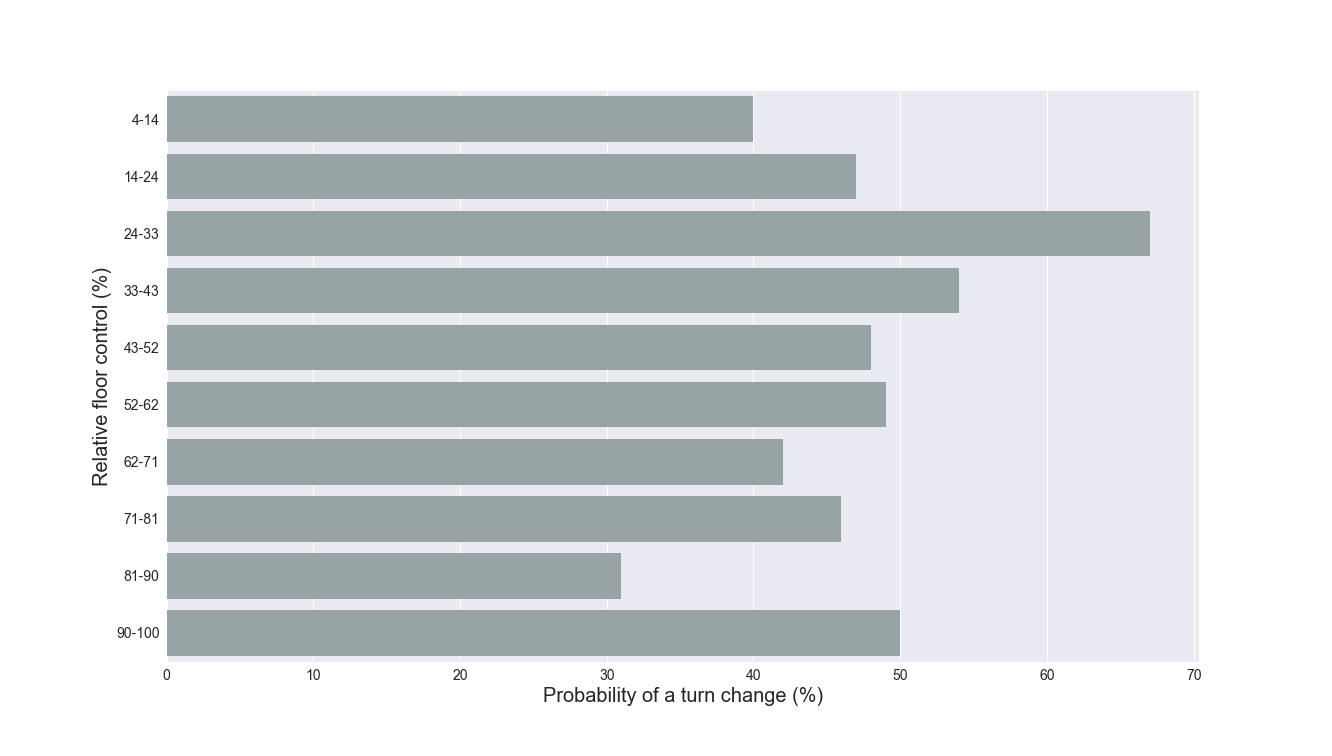
\includegraphics[width=36em]{../scikitlearn/figures/f6.png}\vspace{-1em}
\end{figure}
\end{frame}

\begin{frame}{Relative turn length for dialog act type}
\begin{figure}[ht!]
\centering
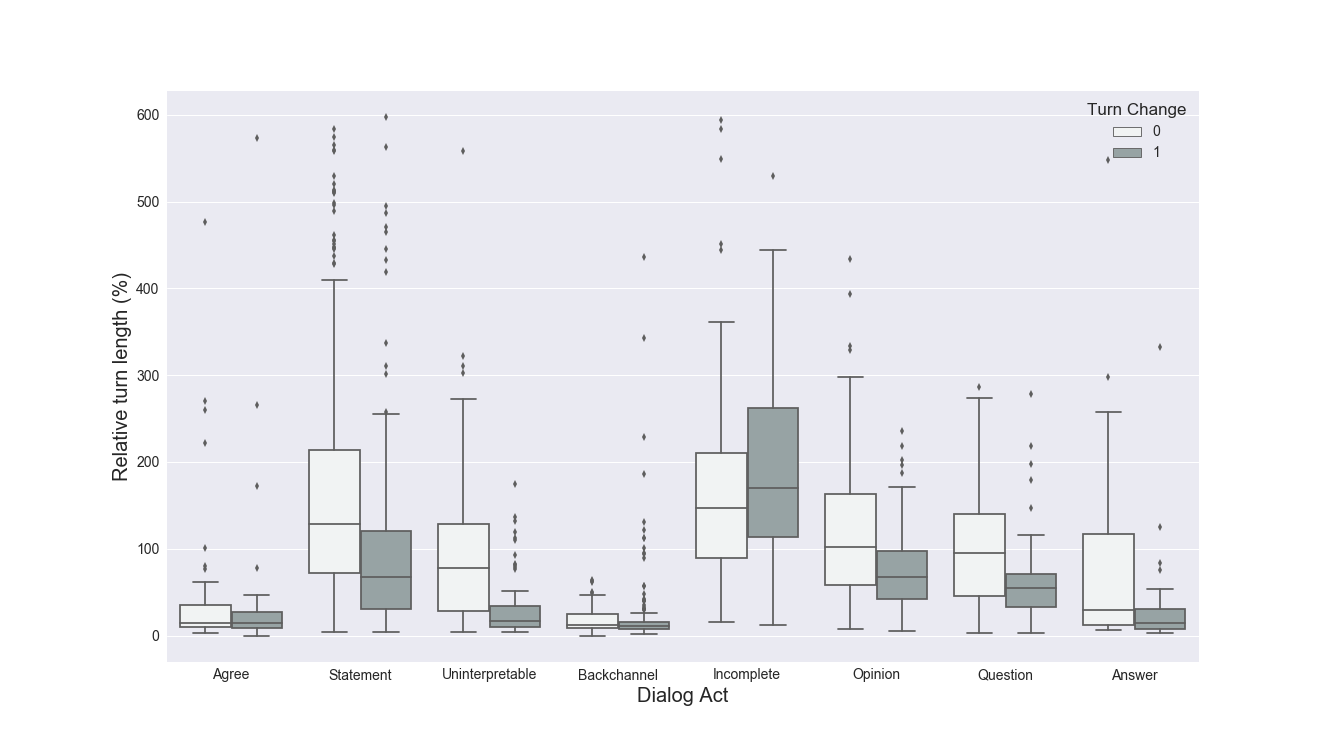
\includegraphics[width=36em]{../scikitlearn/figures/f3.png}\vspace{-1em}
\end{figure}
\end{frame}


\begin{frame}{Relative floor control by dialog act}
\begin{figure}[ht!]
\centering
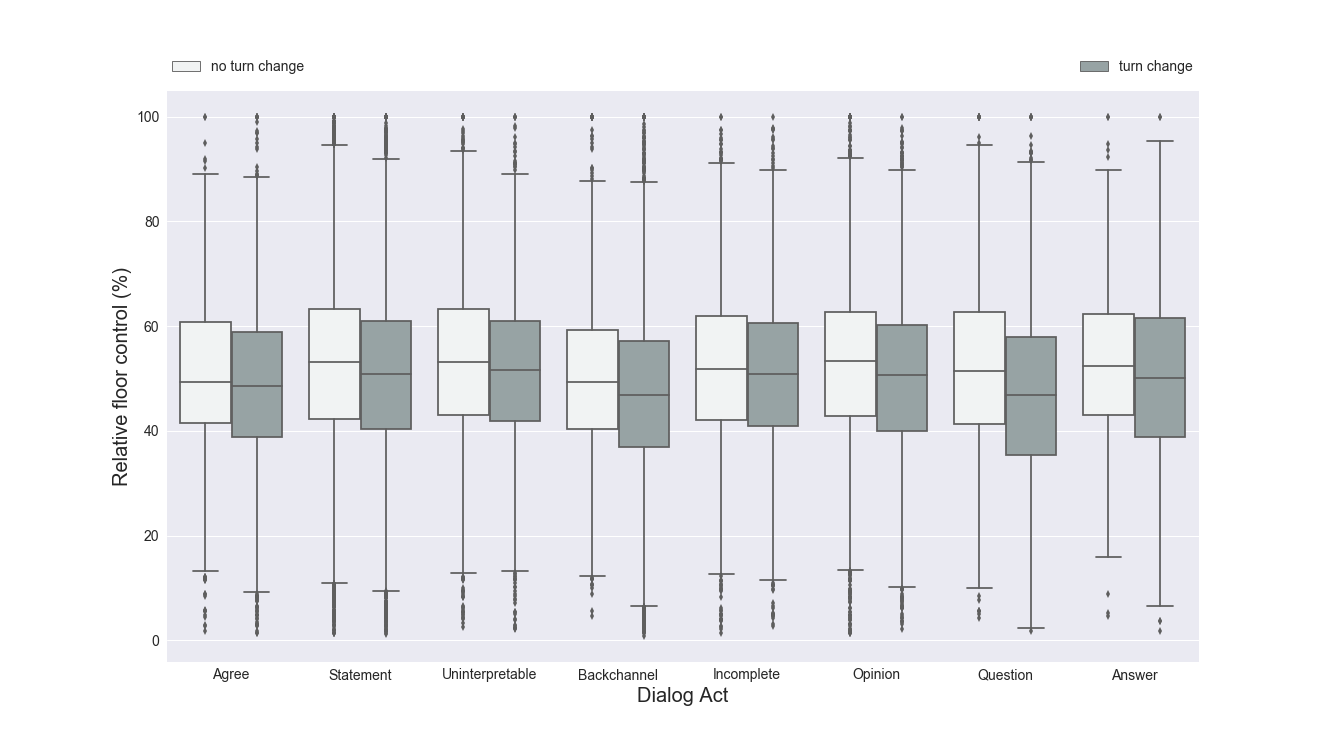
\includegraphics[width=36em]{../scikitlearn/figures/f4.png}\vspace{-1em}
\end{figure}
\end{frame}
